% *********************************************************************
% © 2026 Jeremy Sylvestre
%
% Permission is granted to copy, distribute and/or modify this document
% under the terms of the GNU Free Documentation License, Version 1.3 or
% any later version published by the Free Software Foundation; with no
% Invariant Sections, no Front-Cover Texts, and no Back-Cover Texts. A
% copy of the license is included in the appendix entitled “GNU Free
% Documentation License” that appears in the output document of this
% PreTeXt source code. All trademarks™ are the registered® marks of
% their respective owners.
%
% *********************************************************************
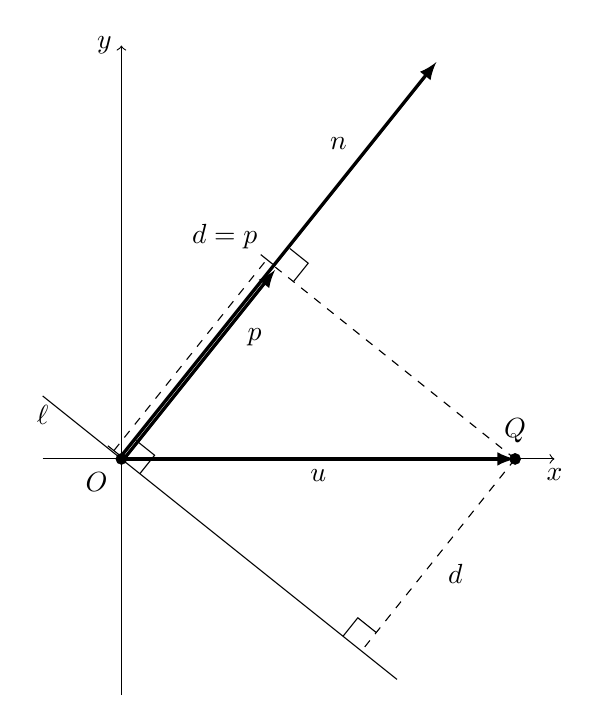
\begin{tikzpicture}[
	vector/.style={-latex,very thick},
	point/.style={circle,draw,very thin,fill,inner sep=0pt,minimum size=4pt},
	% scale=0.75
]
	% projection
	\coordinate (o) at (0,0);
	\coordinate (Q) at (5,0);
	\coordinate (n) at (4,5);
	\coordinate (p) at (1.951,2.439);
	\coordinate (foot) at (3.049, -2.439);

	\draw[->] (-1,0) to (5.5,0) node[below] {$x$};
	\draw[->] (0,-3) to (0,5.25) node[left] {$y$};

	% parallel to (5,-4)
	\draw[thin] (-1,0.8) to node[below,at start] {$\ell$} (3.5,-2.8);

	\node[point] at (o) [label=below left:$O$] {};
	\node[point] at (Q) [label=above:$Q$] {};

	\draw[vector] (o) to node[below] {$\uvec{u}$} (Q);
	\draw[vector] ([yshift=0.04cm]o) to node[above left,near end] {$\uvec{n}$} ([yshift=0.04cm]n);
	\draw[vector] ([yshift=-0.04cm]o) to node[below right,near end] {$\uvec{p}$} ([yshift=-0.04cm]p);
	\draw[dashed] (Q) to (p);
	\draw[dashed,|-|] ([xshift=-0.1cm,yshift=0.1cm]o) to node[above left,at end] {$d = \unorm{p}$} ([xshift=-0.1cm,yshift=0.1cm]p);
	\draw[dashed] (Q) to node[below right] {$d$} (foot);

	% perp symbol
	\draw[thin,rotate=-38.66] (0.3,0) to (0.3,0.3) to (0,0.3);
	\begin{scope}[xshift=1.951cm,yshift=2.439cm]
		\draw[thin,rotate=-38.66] (0.3,0) to (0.3,0.3) to (0,0.3);
	\end{scope}
	\begin{scope}[xshift=3.049cm,yshift=-2.439cm]
		\draw[thin,rotate=-38.66] (-0.3,0) to (-0.3,0.3) to (0,0.3);
	\end{scope}

\end{tikzpicture}
